\chapter{Background}
\label{ch:background}
This chapter contains some of the background material that serves as the basis for this thesis, with additional related work listed in Ch.~\ref{ch:related_work}. 


\section{Software Modeling and Modeling Languages}
\label{sec:software_modeling}
In the world of software development, potential problems and challenges that may arise when developing a product are plentiful. In anything but trivial systems, bugs are almost inevitable, and may be caused by anything from plain programming errors to intermittent problems as a result of resource contention. Systems with concurrent behavior are particularly difficult to implement sensibly, as there are several additional complexities and pitfalls associated with these. Potential problems are also not only related to bugs, but possibly also performance and correctness.

\noindent
In addition to many types of software being nontrivial to implement, keeping the code \emph{readable} is an undertaking of its own. When new developers are added to a team that is already deep into the development process, it can take significant time and effort to become familiar with the system. This can be a result of several factors, such as different code styles, massive spread of code (over a vast amount of files or classes), or simply bad code. In many cases, we may also want non-programmers, such as customers or salespeople, to understand what the system does.

\noindent
Software modeling serves as a solution for smoothing out these processes. Instead of the system specification existing only as code a list of functionality and bugs, it is possible to create a visual and formal model of the system. Such models are more readily understood by non-programmers, and also help other developers become familiar with the overall system architecture more quickly.

\subsection{The Purpose of Software Modeling}
\label{sec:software_modeling_purpose}
The real world is often complex, and correctly expressing this complex world in terms a computer can understand is not a trivial task. Software modeling in languages such as \gls{uml} or \gls{sdl} is a useful tool, helping smooth out this process in several ways.

\paragraph{Conceptual Abstractions} The most important purpose of software models is perhaps to provide \emph{conceptual abstractions}, by describing system functionality and collaborations on a higher level, removing less relevant detail~\cite{braek:itut_methodologies}. This allows developers and other interested parties to get a clear overview of the system architecture, without having to dig through thousands of lines of code.

\paragraph{Separation of Concerns} Another purpose of software modeling is \emph{separation of concerns}, which involves reducing the perceived complexity of the system by modeling parts that are fairly independent as separate, but collaborating, entities~\cite{braek:itut_methodologies}. This may also allow the system to be modularized, potentially simplifying both implementation and maintenance of the system.

\paragraph{Formal Analysis} With the use of formal and well-established modeling methods, we also open up the system design to formal analysis. Depending on the method, we may be able to mathematically or logically analyze the system architecture in order to uncover inconsistencies or errors, or calculate additional system requirements such as hardware capabilities or bandwidth.


TODO



\subsection{UML Activities}
\label{sec:uml_activities}
The \gls{uml} Activity diagram is a modeling concept suitable for expressing processes and workflows, particularly where concurrent behavior is observed. \gls{uml} Activities use \emph{Petri-net-like} semantics, and can be mathematically verified in various ways~\cite{eshuis:uml_verification, storrle:uml_verification}.

\noindent
In general, \gls{uml} Activity diagrams may consist of a number of different types of elements. These include, among others, logical elements such as \emph{forks} and \emph{joins}, allowing concurrent execution and synchronization of these. Other examples are \emph{decisions}, implementing alternate branches, and \emph{wait nodes}, allowing the application to wait for an event before continuing execution.  The activity is executed as a series of \emph{activity steps}, where each step involves performing the logic of one or more elements. An example of a \gls{uml} Activity diagram containing many of these elements is displayed in Fig.~\ref{fig:activity_diagram}.

\begin{figure}[htp]
	\centering
	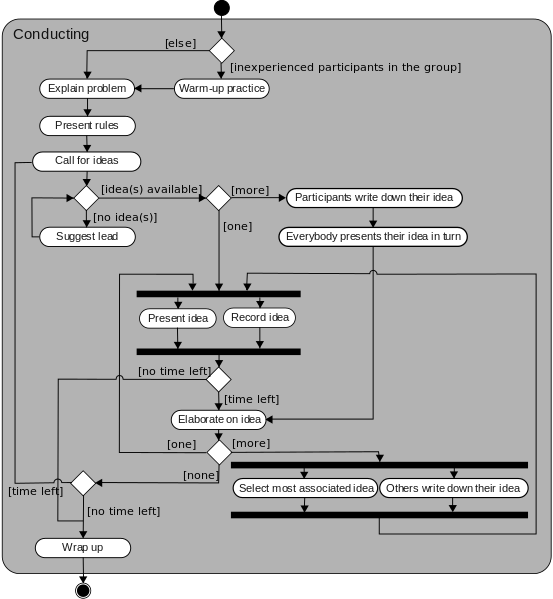
\includegraphics[width=0.8\textwidth]{activity_diagram}
	\caption[UML Activity Diagram]{An UML Activity diagram for a brainstorming process. The process consists of various \emph{actions}, such as ``Explain problem'' or ``Present idea'', that are separated primarily by conditional logic through \emph{decisions}. We also see some examples of concurrent behavior with synchronization, more specifically before and after the ``Present idea'' and ``Record idea'' actions. Both actions are performed simultaneously, and execution does not continue until both actions have finished. We also see the start and end points of activity execution, the \emph{initial node} and the \emph{final node}, as the two black circles above and below the gray area. \emph{Image source: \url{http://en.wikipedia.org/wiki/Activity_diagram}}}
	\label{fig:activity_diagram}
\end{figure}

\subsection{Model-Driven Development}
\label{sec:model_driven_development}
realization is separate from functionality

\section{Tutorials}
\label{sec:tutorials}
TODO: mention more about tutorials in games \\
``A tutorial is a method of transferring knowledge and may be used as a part of a learning process. More interactive and specific than a book or a lecture, a tutorial seeks to teach by example and supply the information to complete a certain task.''~\cite{wiki:tutorial}

\noindent
Tutorials are often used to teach and introduce new topics to users who previously have little or no experience with it. Tutorials may be designed for learning a vast range of topics, such as:
\begin{itemize}
	\item Programming, or using specific programming or modeling languages.\footnote{\url{http://docs.oracle.com/javase/tutorial/}}$^{,}$\footnote{\url{http://www.tutorialspoint.com/uml/}}
	\item Spoken languages.\footnote{\url{http://ielanguages.com/}}
	\item Software products.\footnote{\url{http://www.photoshoptutorials.ws/category/photoshop-tutorials/}}
	\item Video games (such tutorials are usually presented inside the game itself)
	\item Real-life skills, like photography.\footnote{\url{http://photography.tutsplus.com/}}
	\item Human sciences.\footnote{\url{http://anthro.palomar.edu/tutorials/}}
\end{itemize}

\noindent
The above list is in no way exhaustive, but meant to offer some examples of the numerous and diverse topics that may be introduced with the help of a tutorial. In the following chapters, we are primarily concerned with tutorials for programming, software products and video games.

\noindent
Additionally, tutorials come in many forms. The most common form of tutorial is likely the text-based tutorial, often supplemented by illustrations and pictures, but tutorials also come in the form of videos, animations, audio, or in the case of many video games, an interactive experience combining any or all of these.

\noindent
The term ``tutorial'' also defines a concept in the context of British (and other) academia, which is a small class tutored by a lecturer. This type of tutorial is not relevant to this thesis and will not be considered further.

\subsection{Why Do We Use Tutorials?}
\label{sec:tutorial_why}
TODO

\subsection{The Structure of a Tutorial}
\label{sec:tutorial_structure}
Tutorials for different types of topics are generally structured in a way the author believes will provide a good introduction for the given topic, starting with the necessary basic information, and then building on this to learn more advanced concepts. Depending on both the topic and the author, this may result in very different structures.

\noindent
Looking at some of the examples from Sect.~\ref{sec:tutorials}, we see that while the Java tutorials provide stepwise instructions for reaching a specific goal, the spoken language tutorials serve as more of a lookup reference for the most basic concepts within the language. The spoken language tutorials are actually in some ways similar to the separate Java API documentation.\footnote{\url{http://docs.oracle.com/javase/8/docs/api/index.html}}

\noindent
While there are differences in how tutorials for various topics are made, we can identify some general patterns and elements that are present in a wide range of different tutorials:
\begin{itemize}
	\item A list of prerequisites, such as knowledge, equipment or both.
	\item Basic and/or advanced information about the topic, depending on the scope of the tutorial. Often presented in a stepwise manner, starting from the most basic and moving on to the more advanced.
	\item Examples on how to use the information provided in specific cases or contexts.
	\item Exercises where the reader must try to use the concepts introduced in a specific context. Often the whole tutorial is designed as an exercise, presented as a series of steps the user must complete.
	\item Illustrations, figures, or animations, providing the reader with additional examples, information about concepts, or desired results from exercises.
	\item Some kind of motivation for learning about the topic, often as part the tutorial introduction.
\end{itemize}

\noindent
In various combinations, these elements aim to make the introduction to a topic more progressive and intuitive for new users.

\noindent
It is also worth noting that most topics are rarely introduced by a single tutorial. A tutorial is more often designed to introduce only a specific concept within or a part of a topic, with additional tutorials covering other parts. This allows the user to first become familiar with basic concepts, before moving on to tutorials covering the more advanced parts.

\subsection{The Characteristics of a Tutorial}
\label{sec:tutorial_characteristics}


\paragraph{Presence} 

\paragraph{Context-sensitivity}

\paragraph{Degree of freedom}

\paragraph{Help-on-demand}
 


%\subsection{What Makes a Tutorial Good?}
%https://www.udemy.com/blog/how-to-make-a-great-tutorial-video/
%http://spyrestudios.com/the-anatomy-of-a-great-tutorial/
%http://www.gamasutra.com/view/feature/134774/the_designers`_notebook_eight_.php
%http://chris.pirillo.com/how-to-make-a-great-video-tutorial/
%http://menwithpens.ca/great-tutorial/


\section{Learning Programming and Software Modeling}
\label{sec:learning_programming}
In order to teach potential users to use topics such as a programming language, paradigm, protocol or modeling language, various tools or sources of information may be provided. Generally, some form of formal documentation or specification of the language or protocol is considered mandatory, and serves as the \emph{definitive} source of information. Additionally, various tutorials and exercises are often created in order to provide a better introduction to the topic, decreasing the threshold for learning this topic.

\subsection{Documentation}
While a topic's documentation often serves as its primary source of information, such formal documents are not necessarily the best source of information when \emph{learning} about the given topic. Often it is not intended as a learning resource, but rather as a formal reference for users already familiar with the topic. In the documentation, the topic is generally presented in a structured way with respect to its various aspects, so that it is easy for someone already familiar with the topic to find the required information.

\noindent
A good example of this is the \gls{uml} specification.\footnote{\url{http://www.omg.org/spec/UML/2.4.1/}} While the specification offers detailed information about every aspect of \gls{uml} in a way that suits an experienced user, it is likely confusing and not particularly helpful for a user with no previous experience or knowledge about \gls{uml}. Using this specification as a starting point for learning \gls{uml} is likely to require a lot of effort from the user. In the worst case, the user may not even learn all the concepts properly, despite the provided information being very specific and accurate.

\noindent
More importantly, the user may not learn how to properly apply the learned concepts to a given situation. In many cases, 


\subsection{Advantages and Challenges}




\section{Game-based learning}
\label{sec:game_based_learning}

\subsection{Gamification}


\subsection{Learning Inside the Game}


\subsection{Applying Acquired Knowledge and Skills in the Game}






